\documentclass[fleqn,usenatbib]{mnras}

\usepackage{newtxtext,newtxmath}
\usepackage[T1]{fontenc}
\DeclareRobustCommand{\VAN}[3]{#2}
\let\VANthebibliography\thebibliography
\def\thebibliography{\DeclareRobustCommand{\VAN}[3]{##3}\VANthebibliography}


%%%%% PACKAGES %%%%%
\usepackage{amsmath}
\usepackage{graphicx}
\usepackage{aliascnt}
\usepackage{enumitem}
\usepackage{xcolor}
\usepackage{hyperref}
\usepackage{gensymb}
\usepackage{CJK}
\usepackage{tabularx}
\usepackage{orcidlink}
\usepackage{fontawesome}
\usepackage[normalem]{ulem}
\hypersetup{
    unicode, 
    colorlinks=true,
    linkcolor=linkcolor,
    citecolor=linkcolor,
    filecolor=linkcolor,
    urlcolor=linkcolor,
}
\definecolor{linkcolor}{rgb}{0.0,0.3,0.5}

%%%%% COMMANDS %%%%%
\newcommand{\SB}[1]{{\textcolor{purple}{SB: #1}}}
\newcommand{\comment}[1]{\textcolor{lightgray}{#1}}

\newcommand{\asa}{\textcolor{teal}}
\newcommand{\asac}[1]{\color{teal}[ÁS: #1] \color{black}}
\newcommand{\asams}[1]{\textcolor{magenta}{\sout{#1}}}
\newcommand{\asam}{\textcolor{magenta}}
\newcommand{\asas}[1]{\textcolor{teal}{\sout{#1}}}
\newcommand{\mkn}[1]{\textbf{\textcolor{blue}{MKN: #1}}}

\defcitealias{Buder2025c}{Paper~I}

%%%%%%%%%%%%%%%%%%%%%%%%%%%%%%%%%%%%%%%%%%%%%%%%%
%%%%%%%%%%%%%%%%%%%%%%%%%%%%%%%%%%%%%%%%%%%%%%%%%
% \begin{document}
\title[Were Splash stars heated or already born hot?]{The chemodynamical memory of a major merger in a NIHAO-UHD\thanks{NIHAO-UHD is the Ultra High Definition re-run of a Milky Way analogue from the \textit{Numerical Investigation of a Hundred Astronomical Objects} (NIHAO) suite \citep{Wang2015}.} Milky Way analogue II: Were Splash stars heated or already born hot?}

\author[S. Buder et al.]{Sven Buder,$^{1}$\thanks{E-mail: sven.buder@anu.edu.au}\thanks{Australian Research Council DECRA Fellow}\orcidlink{0000-0002-4031-8553}
Tobias Buck,$^{2,3}$\orcidlink{0000-0003-2027-399X}
Ása Skúladóttir,$^{4}$\orcidlink{0000-0001-9155-9018}
Melissa Ness,$^{1}$\orcidlink{0000-0001-5082-6693}
Madeleine McKenzie,$^{5}$\thanks{NASA Hubble Fellow}\orcidlink{0000-0002-1715-1257}
and\newauthor
Stephanie Monty$^{6, 7}$\orcidlink{0000-0002-9225-5822}
\\
$^{1}$Research School of Astronomy and Astrophysics, Australian National University, Canberra, ACT 2611, Australia\\
$^{2}$Universit{\"a}t Heidelberg, Interdisziplin{\"a}res Zentrum f{\"u}r Wissenschaftliches Rechnen, Im Neuenheimer Feld 205, D-69120 Heidelberg, Germany\\
$^{3}$Universit{\"a}t Heidelberg, Zentrum f{\"u}r Astronomie, Institut f{\"u}r Theoretische Astrophysik, Albert-Ueberle-Straße 2, D-69120 Heidelberg, Germany\\
$^{4}$Dipartimento di Fisica e Astronomia, Universitá degli Studi di Firenze, Via G. Sansone 1, I-50019 Sesto Fiorentino, Italy\\
$^{5}$The Observatories of the Carnegie Institution for Science, 813 Santa Barbara Street, Pasadena, 91101, CA, USA\\
$^{6}$Institute of Astronomy, University of Cambridge, Madingley Road, Cambridge CB3 0HA, UK\\
$^{7}$Department of Astronomy, New Mexico State University, Las Cruces, NM 88003, USA
}

% These dates will be filled out by the publisher
\date{Accepted 2025 Month DD. Received 2025 Month DD; in original form 2025 October 15}

% Prints the current year, for the copyright statements etc. To achieve a fixed year, replace the expression with a number. 
\pubyear{\the\year{}}

% Don't change these lines
\begin{document}
\label{firstpage}
\pagerange{\pageref{firstpage}--\pageref{lastpage}}
\maketitle

\begin{abstract} % 181 words, 1388 characters with space
One of the most debated consequences of the Milky Way's last major merger is the so-called \textit{Splash}: stars with disc-like chemistry but halo-like kinematics, often interpreted as evidence for the violent heating of an early protodisc. Using the same high-resolution NIHAO-UHD cosmological simulation analysed in Buder et al. (2025b, hereafter Paper I), we test whether, and if so how, a Splash-like population arises in the Milky Way analogue. By tracing stellar birth positions, ages, and present-day orbits, we find that protodisc stars were already born on dynamically hot orbits. We find no evidence for significant additional dynamical \textit{splashing} of in-situ stars despite a 1:5 stellar mass merger. The observed Splash may therefore reflect the already turbulent early disc, subsequently intermixed with accreted stars and those formed from merger-driven gas inflows, rather than a distinct merger-heated population. When selecting Splash stars via chemistry and age, we find their azimuthal velocity distribution to be distributed across a wider range and positively skewed with $V_\varphi = 73_{-59}^{+74}\,\mathrm{km\,s^{-1}}$. The transition of the stellar disc to a rotation-supported one with large azimuthal velocities occurs only during or after the merger. Our results suggest an alternative to the proposed splashing, and highlight the need to disentangle the relative contributions of merger-induced heating and intrinsically hot disc formation in order to clarify the nature of Splash-like stars and their role in shaping the early Milky Way.
\end{abstract}

\begin{keywords}
% {
Galaxy: evolution -- Galaxy: formation -- Galaxy: structure -- Galaxy: abundances -- Galaxy: kinematics and dynamics
% }
\end{keywords}

% \maketitle

%%%%%%%%%%%%%%%%%%%%%%%%%%%%%%%%%%%%%%%%%%%%%%%%%
%%%%%%%%%%%%%%%%%%%%%%%%%%%%%%%%%%%%%%%%%%%%%%%%%
\section{Introduction}
\label{sec:introduction}

A long-standing goal of Galactic archaeology is to reconstruct how mergers shaped the early Milky Way. Thanks to \textit{Gaia} astrometry \citep{Brown2021b} and large spectroscopic surveys \citep{Jofre2019}, it is now clear that our Galaxy experienced at least one major accretion event about 8--10~Gyr ago, commonly referred to as the \textit{GSE} merger \citep{Haywood2018b, Belokurov2018, Helmi2018, Naidu2020}. This event left an imprint in the stellar halo, and growing evidence suggests that it also influenced a pre-existing disc, dynamically mixing the earliest in-situ populations with accreted debris \citep{Helmi2020}.

One of the most debated signatures of this process is the so-called Splash population \citep{Belokurov2020, Belokurov2022}. These stars appear chemically similar to the old, $\upalpha$-enhanced thick disc, but occupy hotter, halo-like orbits. Their dual nature has made them central to arguments about whether the \textit{GSE} merger violently heated the protodisc, or whether some old stars were already born on dynamically hot orbits in our Galaxy’s turbulent youth.

Observational studies first pointed to an in-situ halo component overlapping with the disc in chemistry. \citet{Bonaca2017} identified metal-rich, prograde halo stars consistent with a heated thick disc origin. Expanding on this, \citet{Bonaca2020} used \textit{Gaia} DR2 and H3 survey data to argue that disc-like chemistry but halo-like kinematics reflect merger-driven heating, providing a timeline for disc perturbation shortly after \textit{GSE}. Similarly, \citet{DiMatteo2019,DiMatteo2020} interpreted metal-rich, eccentric stars as evidence that the \textit{GSE} merger dynamically heated pre-existing disc stars into the halo, strengthening the case that Splash stars trace this violent epoch.

Other studies have argued for alternative or complementary origins. In a hydrodynamical simulation of an isolated clumpy disc, \citet{Amarante2020} showed that a Splash-like component can form without mergers: stars scattered by giant clumps during early, turbulent disc phases naturally occupy low-angular-momentum, halo-like orbits, yet remain chemically continuous with the thick disc. More recently, cosmological simulations have broadened the picture. \citet{Dillamore2022} found that Splash-like stars could be a generic feature of Milky Way analogues, while \citet{Dillamore2023} showed that bar resonances can also create halo-like substructures. Extending this, \citet{Dillamore2025} demonstrated that secular evolution can reshape integral-of-motion space, complicating attempts to uniquely attribute Splash stars to merger heating. Observationally, \citet{Kisku2025} showed that Splash stars occupy the high-$\alpha$, high-[Al,K/Fe], low-[Mn/Fe] extension of the thick disc sequence, and, in combination with ARTEMIS simulations \citep{Font2020}, argued that both major and minor mergers can produce Splash-like signatures, in agreement with the conclusions from the HESTIA simulation by \citet{Khoperskov2023}. A complementary, physically explicit pathway is feedback-driven \textit{baryon sloshing} in gas-rich discs, which isotropically heats newly formed stars and builds a thick disc without requiring a contemporaneous major heating event \citep{BlandHawthorn2025}

Taken together, these studies highlight that Splash stars remain a crucial but unresolved tracer of the Milky Way’s formative history. They may represent violently heated disc stars, stars born hot in a turbulent proto-disc, or a mixture of both, possibly reshaped by subsequent secular evolution. The distinction matters: if Splash stars are heated, they provide a dynamical clock for the last major merger; if they are born hot, they instead reflect the conditions of the early disc, independent of mergers.

In \citet[][hereafter Paper~I]{Buder2025c}, we used a NIHAO-UHD cosmological simulation of a Milky Way analogue \citep{Buck2020, Buck2021} to examine the chemodynamical memory of a major merger. \citetalias{Buder2025c} focused on the efficiency of recovering accreted stars in integral-of-motion space, the preservation of their birth radii, and chemical evolution. Building on this framework, this work (Paper~II) asks whether a Splash-like population emerges in a fully cosmological Milky Way analogue, and if so, whether these stars were \emph{heated by the merger or already born hot}. Our guiding questions are:
\begin{enumerate}[leftmargin=2em,labelwidth=0em]
    \item Does a distinct Splash population emerge in a high-resolution cosmological simulation?
    \item Is this population born in the Milky Way analogue or also/only the \textit{GSE}-like galaxy that merged with it around $8.6\,\mathrm{Gyr}$ ago?
    \item Are Splash-like stars dynamically heated, or do they form already hot in the turbulent early disc?
    \item What does the simulated Splash imply for interpreting the Milky Way’s merger-driven history?
\end{enumerate}

%%%%%%%%%%%%%%%%%%%%%%%%%%%%%%%%%%%%%%%%%%%%%%%%%
%%%%%%%%%%%%%%%%%%%%%%%%%%%%%%%%%%%%%%%%%%%%%%%%%
\section{Simulation data}
\label{sec:data}

We use the same high-resolution cosmological zoom-in simulation analysed in \citetalias{Buder2025c}, namely the NIHAO-UHD Milky Way analogue \texttt{g8.26e11} \citep{Wang2015, Buck2019b, Buck2020b, Buck2021}. The simulation was performed with the smoothed-particle hydrodynamics code \texttt{Gasoline2} \citep{Wadsley2017}, following the NIHAO feedback and enrichment framework \citep{Stinson2006, Stinson2013, Wang2015}. It adopts a $\Lambda$CDM cosmology as inferred by \citet{Planck2014} and includes metal-line cooling, star formation, and stellar feedback with chemical enrichment from asymptotic giant branch stars, core-collapse supernovae, and supernovae of type Ia \citep{Buck2021}. The NIHAO-UHD suite reaches ultra-high mass resolution; for \texttt{g8.26e11} the stellar particle mass is $7.5 \times 10^3\,\mathrm{M_{\odot}}$.

This simulation was chosen because it closely resembles the Milky Way in its global properties, such as stellar mass and disc-dominated morphology, and experienced a last major merger at a lookback time of $\sim 8.6$~Gyr, broadly consistent with the timing inferred for the Milky Way's \textit{GSE} merger \citep{Helmi2018, Naidu2021}. At $z=0$, the main halo has a virial radius of $R_{200}=206\,\mathrm{kpc}$ and a total mass of $M_{200}=9.1\times10^{11}\,\mathrm{M_\odot}$, including $8.2\times10^{11}\,\mathrm{M_\odot}$ in dark matter, $6.4\times10^{10}\,\mathrm{M_\odot}$ in gas, and $2.3\times10^{10}\,\mathrm{M_\odot}$ in stars. The last major merger progenitor, a \textit{GSE}-like galaxy, had a stellar mass of $\sim 3\times10^9\,\mathrm{M_\odot}$ and a total mass ratio of roughly $1:5$ relative to the host at the time of infall, comparable to empirical estimates for the Milky Way's \textit{GSE} merger \citep[e.g.][]{Helmi2018, Naidu2021}.
A key structural property of \texttt{g8.26e11} is that it forms a multi-armed spiral disc but no significant present-day bar \citep{Buder2025}. This means that bar-driven resonances, proposed as a possible driver of the \textit{Splash} by \citet{Dillamore2022, Dillamore2023}, are likely not responsible for the features we analyse here.

A full description of the simulation setup, feedback and enrichment prescriptions, and comparison to Milky Way constraints is given in Sec.~2.1 of \citetalias{Buder2025c}. Sec.~2.2 of \citetalias{Buder2025c} details how we trace the birth positions of stars in discrete $100\,\mathrm{Myr}$ time steps relative to the evolving centre of mass of the main halo. Combined with the orbital energies and actions (Sec.~2.3 of \citetalias{Buder2025c}), which we computed with the \textsc{agama} code \citep{Vasiliev2019b}, this enables us to distinguish in-situ stars from those accreted during mergers, as described in Sec.~3.1 of \citetalias{Buder2025c}.

%%%%%%%%%%%%%%%%%%%%%%%%%%%%%%%%%%%%%%%%%%%%%%%%%
%%%%%%%%%%%%%%%%%%%%%%%%%%%%%%%%%%%%%%%%%%%%%%%%%
\section{Analysis: The merger process and its chemodynamical effects} \label{sec:analysis}


In \citetalias{Buder2025c}, we analysed the NIHAO-UHD Milky Way analogue to classify stars into in-situ and accreted populations, examine their orbital properties and selection efficiency in integrals-of-motion space, and evaluate how well birth positions and chemical evolution are retained as chemodynamical memory. Building on this framework, we now focus on the merger's dynamical effects. Our aim is to assess whether the simulation produces a population analogous to the observationally claimed Splash: stars born in the early disc but dynamically heated onto halo-like orbits, stars formed from merger-driven gas mixing, or stars that may be misclassified accreted populations. By linking these possibilities back to the classification, dynamical, and chemical analyses of \citetalias{Buder2025c}, we investigate whether the Splash emerges as a distinct component or as the overlap of several processes.

\subsection{Infall}

In Fig.~3 of \citetalias{Buder2025c} we studied the birth positions of accreted stars within their host galaxy in timesteps of $0.1\,\mathrm{Gyr}$. The birth positions in the $X_\mathrm{birth}$ vs. $Z_\mathrm{birth}$ plane (Fig.~3b of \citetalias{Buder2025c}) demonstrated that the major merger galaxy followed an almost diagonal merger path. When tracking the orbits of the accreted stars born within $50\,\mathrm{kpc}$ of the main galaxy, we calculate the inclination angle $\theta$ of the merger (with larger inclination meaning a more edge-on rather than face-on trajectory) to be between $34$ and $55\,\mathrm{deg}$, based on a singular value decomposition in three dimensions or a linear fit in $X_\mathrm{birth}$ vs. $Z_\mathrm{birth}$, respectively. This value is roughly comparable to the inclination of $\theta = 30\,\mathrm{deg}$ inferred by \citet{Naidu2021} for the Milky Way's \textit{GSE} merger with simulations with multiple inclination and circularity values. We note that the pattern of stars on significantly more prograde orbits (Fig.~4b of \citetalias{Buder2025c}) matches less well with the patterns of typically low absolute angular momenta observed in the Milky Way and simulated for a merger with circularity $\eta = 0.5$. Our orbit pattern rather matches the simulation outcome by \citet{Naidu2021} for a highly circular galaxy with $\eta = 0.9$ (see their Fig.~3). We refrain from interpreting this, however, as there are more particular merger parameters that might play an important role for energy and momentum transfer. This includes the path along which the merging galaxy spiralled into the larger galaxy relative to the galactic plane (see $X_\mathrm{birth}$ vs. $Y_\mathrm{birth}$ in Fig.~3a of \citetalias{Buder2025c}), as well as the locations of passages through this plane.
We can, however, study the kinematic/dynamical effect on already born in-situ stars as well as the chemodynamic effect on stars that formed during the merger.

\begin{figure}
    \centering
    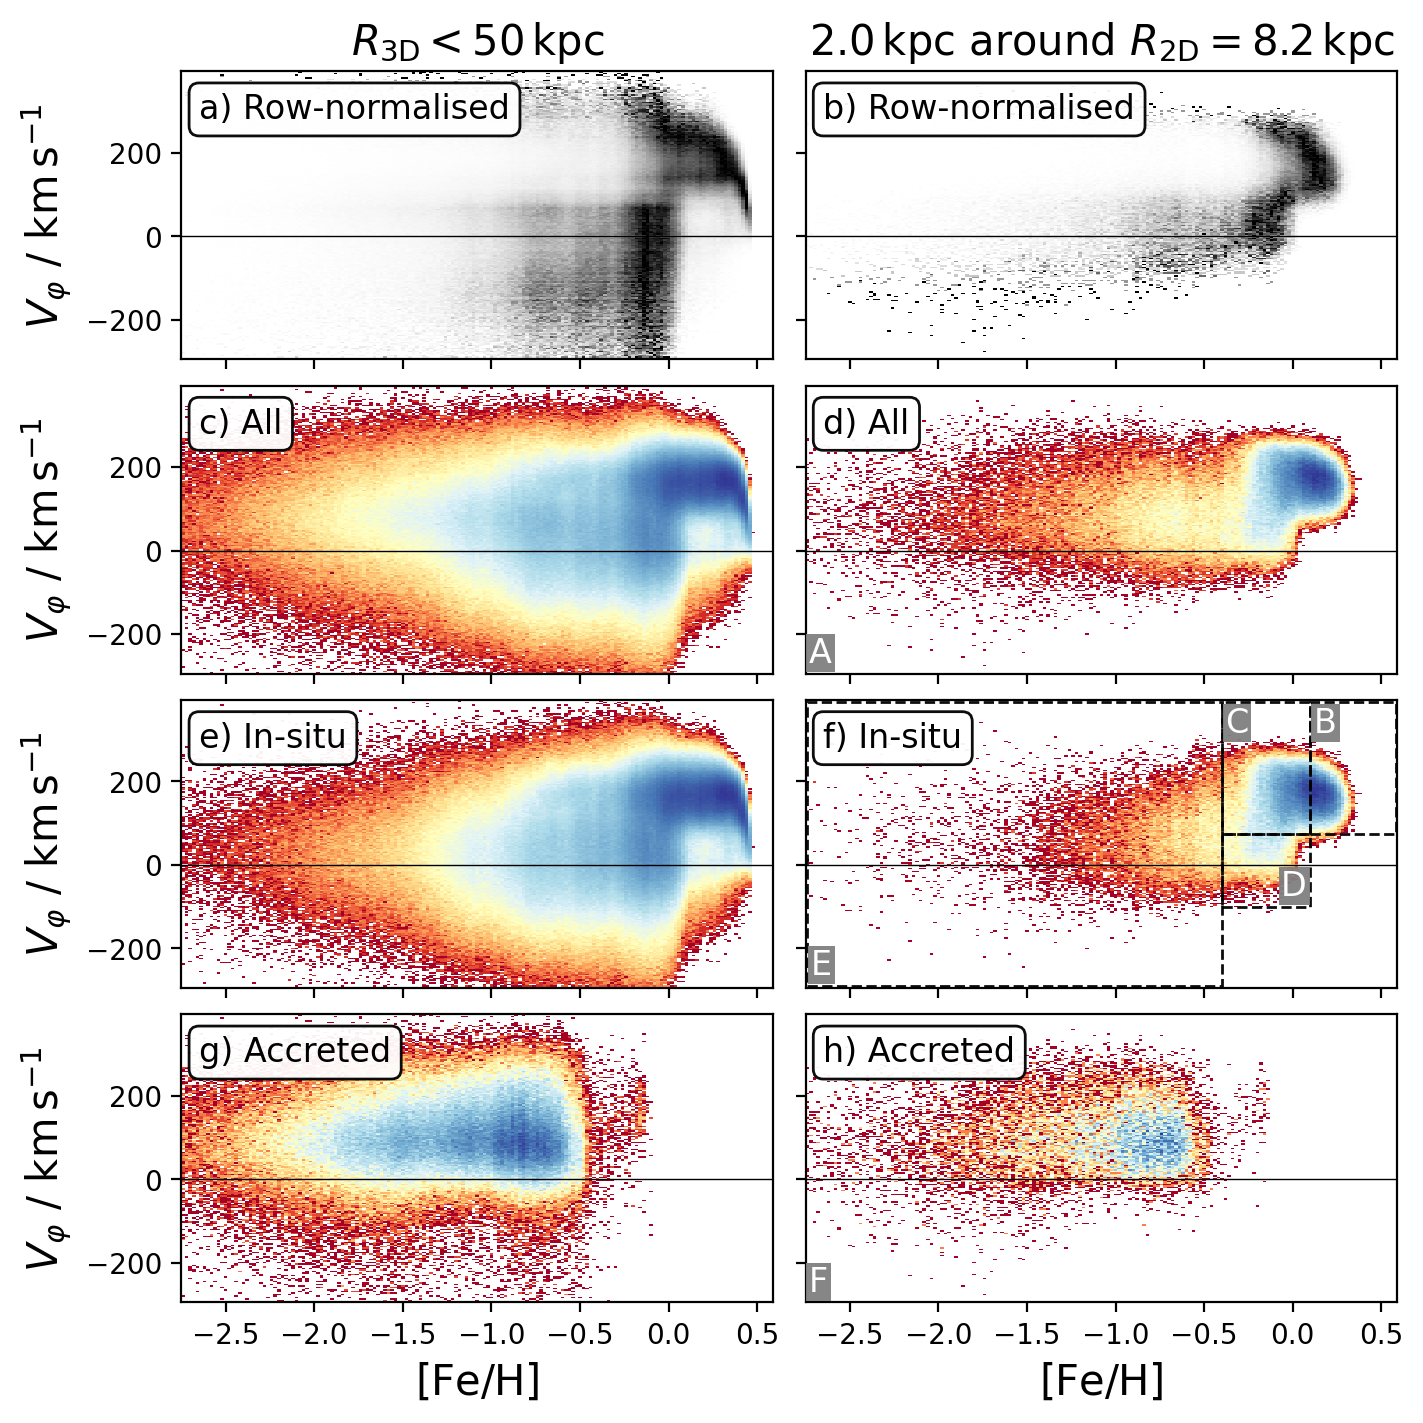
\includegraphics[width=\columnwidth]{figures/splash_feh_vphi.png}
    \caption{{Iron abundance [Fe/H]} vs. azimuthal velocity $V_\varphi$ for stars within $R_\mathrm{3D} < 50\,\mathrm{kpc}$ (left panels) and the Solar-like locus (right panels). Panels a) and b) show the density distribution, when normalising the density across each row, as done by \citet[][see their Fig~1]{Belokurov2020}. Panels c) and d) show the logarithmic density distribution of all stars. Panels e) and f) show in-situ stars, while panels g) and h) show accreted stars. Dashed black rectangles with letters A-F at their lower left corner annotate the selection of different subsamples of the Solar neighbourhood \href{https://github.com/svenbuder/gse_nihaouhd/tree/main/figures}{\faGithub}.}
    \label{fig:splash_feh_vphi}
\end{figure}

\subsection{Selection of Splash-like stars}

Based on a population of stars in the Solar neighbourhood that are more metal-rich than typical halo stars yet follow highly eccentric orbits, \citet{Belokurov2020} proposed that these stars originated in the Milky Way’s disc and were \textit{splashed} onto low-angular-momentum orbits during the last major merger. Motivated by this hypothesis, we analyse stars in our Milky Way analogue in the same plane as \citet{Belokurov2020}, namely $\mathrm{[Fe/H]}$ vs. azimuthal velocity $V_\varphi$, both for the entire galaxy and for a Solar neighbourhood-like region (see Fig.~\ref{fig:splash_feh_vphi}).

In a first step, we replicate the density distribution plots in $\mathrm{[Fe/H]}$ vs. $V_\varphi$ space that \citet[][their Fig.~1]{Belokurov2020} used to identify Splash stars. We show both the row-normalised density distribution in Figs.~\ref{fig:splash_feh_vphi}a and \ref{fig:splash_feh_vphi}b as well as the logarithmic density distributions in Figs.~\ref{fig:splash_feh_vphi}c and \ref{fig:splash_feh_vphi}d. Here we indeed find a strikingly similar distribution in $\mathrm{[Fe/H]}$ vs. $V_\varphi$ space to that observed by \citet{Belokurov2020} for the Solar neighbourhood. In particular, we recover the sickle-like distribution of highest densities (black) around $\mathrm{[Fe/H]} \sim -0.25$ in the row-normalised distribution of Fig.~\ref{fig:splash_feh_vphi}b, which \citet{Belokurov2020} attributed to the three zones of thin disc (top), thick disc (middle), and Splash (bottom).

In the other panels of Fig.~\ref{fig:splash_feh_vphi} with logarithmic density distributions, metal-poor in-situ stars exhibit a broad spread in azimuthal velocity, up to $\pm 300\,\mathrm{km\,s^{-1}}$) centred around $V_\varphi = 0\,\mathrm{km\,s^{-1}}$. Both \citet{Yu2023b} and \citet{Chandra2024} described this as the first of three phases of disc evolution, the chaotic bursty phase. As metallicity increases, the stellar density rises and peaks around $-0.4 < \mathrm{[Fe/H]} < 0.1$ for stars with $V_\varphi < 0\,\mathrm{km\,s^{-1}}$. In this metallicity range, we observe a steep increase in the average $V_\varphi$. This the second phase of disc evolution \citep{Chandra2024} is also described as spin-up/bursty-disc phase  \citep{Yu2023b}. Finally, the most metal-rich stars are moving on rotationally supported disc orbits with a narrower distribution of $200 \pm 100\,\mathrm{km\,s^{-1}}$ \citep[the third, thin-disc phase of disc evolution in][]{Yu2023b, Chandra2024}.

In observations, the interpretation of the [Fe/H]-$V_\varphi$ plane is complicated by uncertainties in stellar ages and the unknown birth locations of stars. In contrast, our simulation allows us to overcome these limitations by providing both precise stellar ages and a clear distinction between in-situ and accreted stars. Taking advantage of this, we define several subsamples of the Solar neighbourhood (Sample~A, Fig.~\ref{fig:splash_feh_vphi}d) to probe the nature of the Splash population. Sample D (Fig.~\ref{fig:splash_feh_vphi}f) selects in-situ Splash-like stars with $-0.4 < \mathrm{[Fe/H]} < 0.1$ and $-100 < V_\varphi < 75\,\mathrm{km\,s^{-1}}$.  More generally, we then define:
\begin{itemize}[leftmargin=2em,labelwidth=2em]
    \item Sample A: all stars in the Solar neighbourhood (Fig.~\ref{fig:splash_feh_vphi}d) \\
    and from within this region we sub-select (Figs.~\ref{fig:splash_feh_vphi}f and \ref{fig:splash_feh_vphi}h):
    \item Sample B: more metal-rich in-situ stars ($\mathrm{[Fe/H]} > 0.1$),
    \item Sample C: in-situ stars with Splash-like [Fe/H] but higher $V_\varphi$,
    \item Sample D: the Splash stars themselves,
    \item Sample E: more metal-poor in-situ stars ($\mathrm{[Fe/H]} < -0.4$), and
    \item Sample F: accreted stars in the Solar neighbourhood.
\end{itemize}

While we identify the Splash-like sample D in Fig.~\ref{fig:splash_feh_vphi} at $-0.4 < \mathrm{[Fe/H]} < 0.1$ in the simulation, we note that \citet{Belokurov2020} found it as slightly lower metallicities of $-0.7 < \mathrm{[Fe/H]} < -0.25$ in the Milky Way's Solar neighbourhood. Because of the findings by \citet{Buck2021}, who studied the influence of chemical evolution model choices, such as nucleosynthetic yields, on chemical evolution predictions on NIHAO-UHD simulations, we attribute this absolute offset in [Fe/H] and other abundances mainly to the choices of chemical evolution parameters in the simulation. Because of these abundance offsets, our selection is consistent with the \textit{relative} position of Splash stars in the [Fe/H] vs. $V_\varphi$ diagrams used by \citet{Belokurov2020}, but not identical.

We also note that \citet{Belokurov2020} did not specifically select in-situ stars for their Splash sample. In the Milky Way analogue, however, we only find stars fitting the Splash selection criteria to be born in-situ (compare Figs.~\ref{fig:splash_feh_vphi}f and \ref{fig:splash_feh_vphi}h in the Splash region). We find the accreted stars of the Milky Way analogue moving with higher azimuthal velocities of $V_\varphi = 100_{-70}^{+80}\,\mathrm{km\,s^{-1}}$% within the Solar neighbourhood (Fig.~\ref{fig:splash_feh_vphi}h), as compared to values of $V_\varphi = 20_{-70}^{+100}\,\mathrm{km\,s^{-1}}$ for \textit{GSE} stars within the Milky Way's Solar neighbourhood \citep{Buder2022}.

\subsection{Ages and chemistry of Splash-like stars}

Before we take a look at possible changes to the dynamics and spatial distribution of these stars, we get an idea of their typical ages and chemistry in Figs.~\ref{fig:splash_age} and \ref{fig:splash_alfe_mgmn}, respectively. In both spaces, we find the Splash stars as part of the in-situ sequence. This sequence extends from the oldest  ($11.3_{-0.7}^{+0.9}\,\mathrm{Gyr}$%) and most metal- and [Al/Fe]-poor in-situ stars to younger Splash stars ($9.2_{-0.7}^{+0.7}\,\mathrm{Gyr}$%) with higher [Al/Fe]. From there, the sequence continues to even younger stars ($7.2_{-3.8}^{+1.3}\,\mathrm{Gyr}$%), which have similar [Fe/H] but higher $V_\varphi$ and [Al/Fe] and lower [Mg/Mn]. Finally, it reaches the youngest and most metal-rich in-situ stars ($3.8_{-2.5}^{+2.0}\,\mathrm{Gyr}$%). Furthermore, we note that the accreted stars with ages of $11.2_{-1.7}^{+1.3}\,\mathrm{Gyr}$% are for the most part older or at least as old as the Splash stars. This finding (of F older than D older than C) is consistent with the observations by \citet{Belokurov2020}. In particular, we also find that the Splash-like stars are exclusively old, corroborating that they indeed could come from a Splash-like event. We also note that while there are stars with chemical compositions literally bridging the accreted (blue) and in-situ (red) populations, this bridge\footnote{The region of $-0.2 < \mathrm{[Al/Fe]} < -0.05$ and $\mathrm{[Mg/Mn]} < -0.14$.} connects at the low [Mg/Mn]-end of the Splash star region. As already noted by \citet{Buder2024}, these stars  (less than 1\,\% within the Solar neighbourhood) are likely formed from mixed gas during the merger, but do not contribute significantly (less than 9\,\%) to any of the sub-samples of the simulation's Solar neighbourhood.

More strikingly, we note only a little overlap in the distribution of ages and chemistry of the most metal-poor in-situ stars with the Splash stars within the Solar neighbourhood. The age distribution of the Splash stars (Sample D) is consistent with the oldest stars of the in-situ population with similar [Fe/H] but higher $V_\varphi$ than the Splash stars (Sample C) and shows a similar profile especially for ages of $9-11\,\mathrm{Gyr}$.

This result opens up a number of questions that evolve around how special the Splash stars are -- both in terms of their chemistry as well as their orbits. While \citet{Belokurov2020} favoured a scenario in which the stars have been splashed by a major merger, they also discussed a scenario in which the stars might have been born dynamically hotter with more eccentric orbits. One could for example imagine these stars being the low azimuthal velocity tail of a dynamically hotter early disc. We thus take a closer look at the sample of stars with similar iron abundance ($-0.4 < \mathrm{[Fe/H]} < 0.1$) and the aforementioned ages of $9-11\,\mathrm{Gyr}$.

\begin{figure}
    \centering
    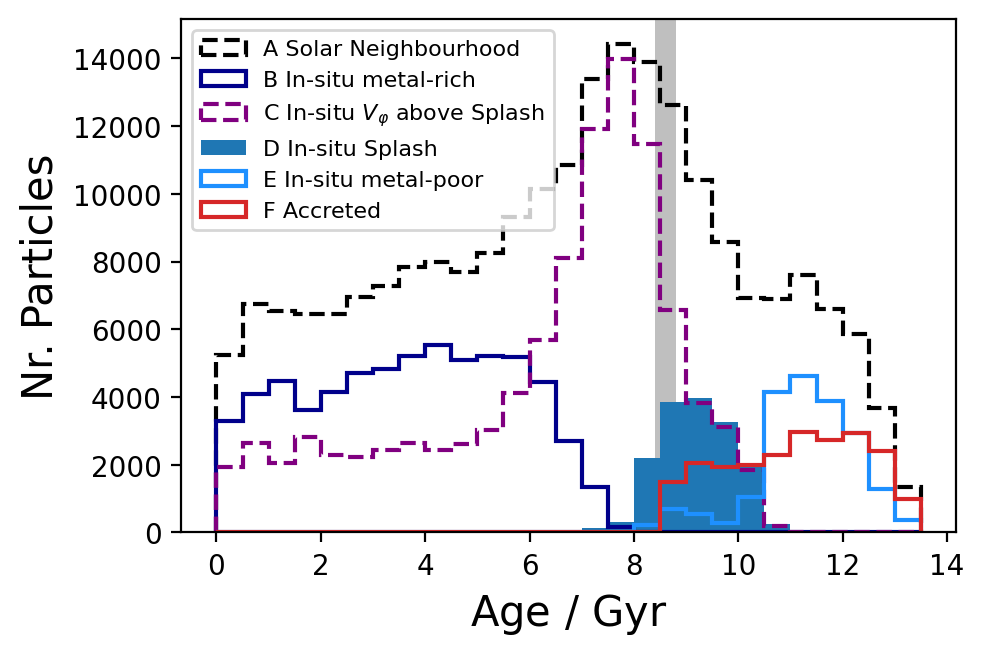
\includegraphics[width=\columnwidth]{figures/splash_age.png}
    \caption{Age distribution of different samples of stars in the Solar neighbourhood as selected in the $\mathrm{[Fe/H]}$ vs. $V_\varphi$ plane of Fig.~\ref{fig:splash_feh_vphi}. A grey bar indicates the time of the major merger around $8.6\,\mathrm{Gyr}$ \href{https://github.com/svenbuder/golden_thread_II/tree/main/figures}{\faGithub}.}
    \label{fig:splash_age}
\end{figure}

\begin{figure}
    \centering
    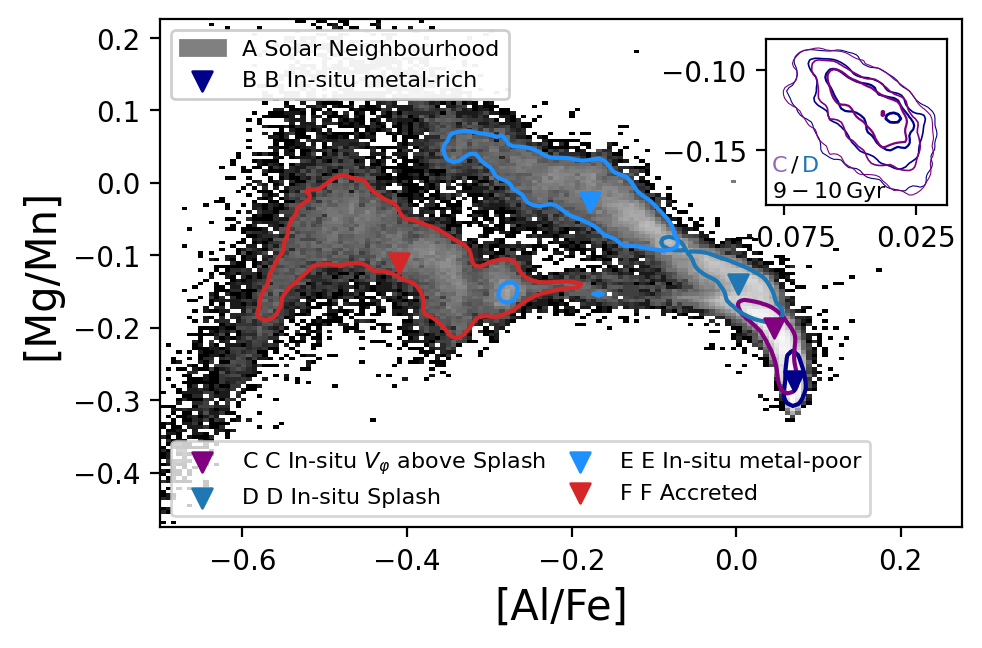
\includegraphics[width=\columnwidth]{figures/splash_alfe_mgmn.png}
    \caption{Abundance distribution in [Al/Fe] vs. [Mg/Mn] of different samples of stars in the Solar neighbourhood as selected in the $\mathrm{[Fe/H]}$ vs. $V_\varphi$ plane of Fig.~\ref{fig:splash_feh_vphi}. Contours correspond to the 68\,\% highest-density interval. An inset figure is showing the distribution of samples C and D with ages of $9-11\,\mathrm{Gyr}$, with contours showing the 40, 60, and 80\,\% highest-density intervals \href{https://github.com/svenbuder/golden_thread_II/tree/main/figures}{\faGithub}.}
    \label{fig:splash_alfe_mgmn}
\end{figure}

\begin{figure}
    \centering
    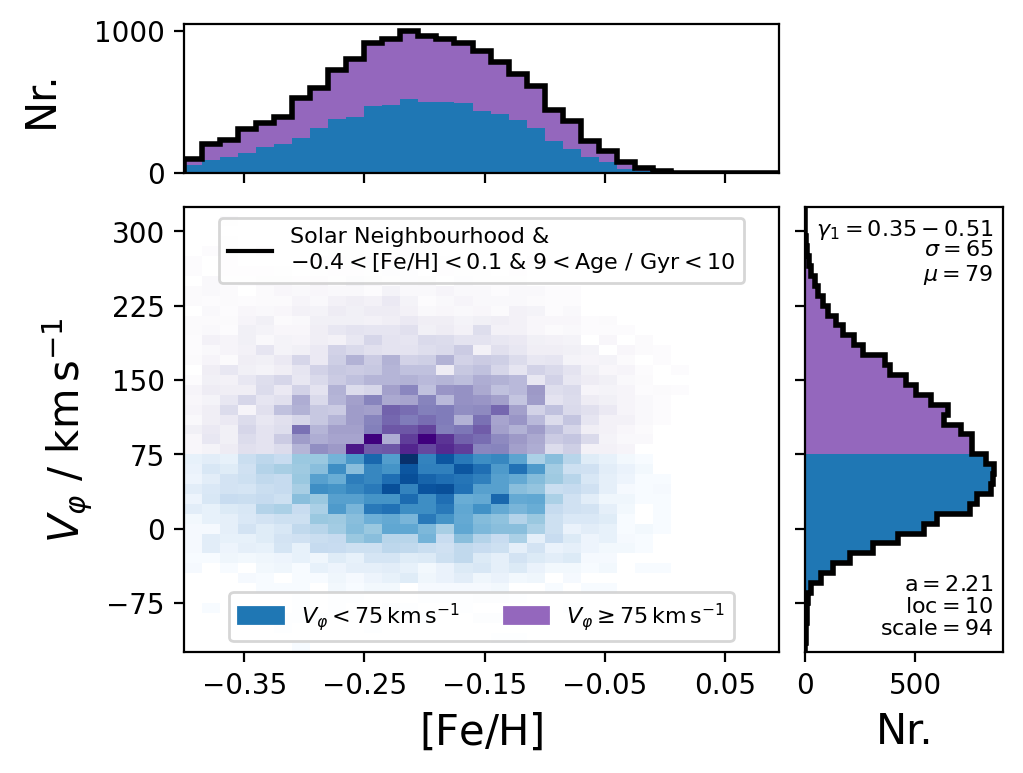
\includegraphics[width=\columnwidth]{figures/splash_vphi_distribution.png}
    \caption{Distributions of [Fe/H] and $V_\varphi$ for stars in the Solar neighbourhood at $-0.4 < \mathrm{[Fe/H]} < 0.1$. We show the stacked distribution (black lines) as well as 2-dimensional and 1-dimensional histograms of each distribution.
    \href{https://github.com/svenbuder/golden_thread_II/tree/main/figures}{\faGithub}.}
    \label{fig:splash_vphi_distribution}
\end{figure}

\begin{figure*}
    \centering
    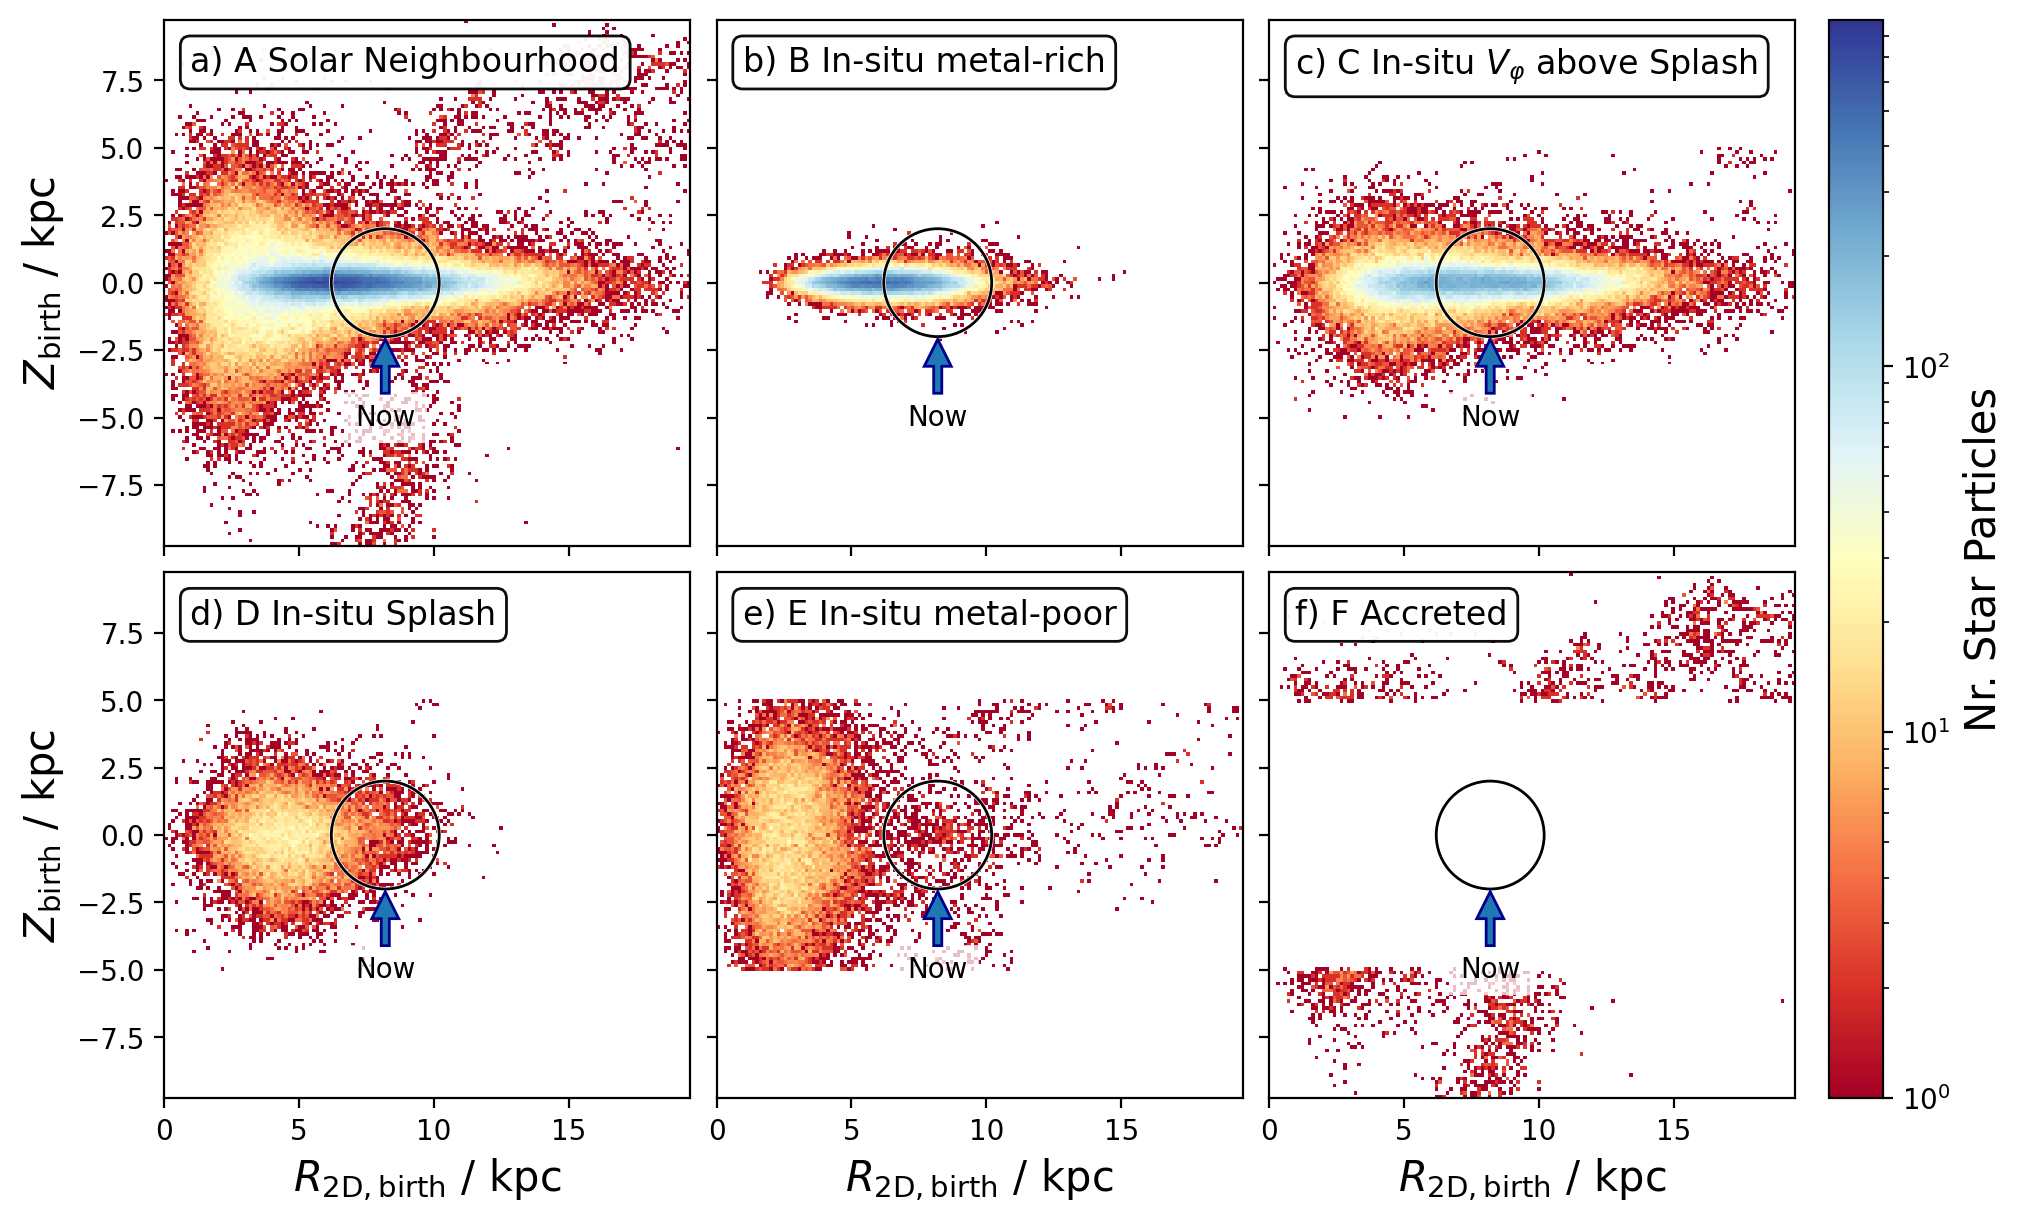
\includegraphics[width=\textwidth]{figures/splash_rbirth_zbirth}
    \caption{Density distribution of birth positions in galactocentric cylindrical coordinates $R_\mathrm{birth, 2D}$ and $Z_\mathrm{birth}$ for star particles of samples A-F (corresponding to panels a-f) that are currently in the Solar neighbourhood (black circles) of $2\,\mathrm{kpc}$ around $R_\mathrm{2D} = 8.2\,\mathrm{kpc}$. In panels e) and f) we note the imprint of our selection of in-situ vs. accreted stars via $\vert Z_\mathrm{birth} \vert > 5\,\mathrm{kpc}$ \citepalias[Eqs.~4 and 5 of][]{Buder2025c} \href{https://github.com/svenbuder/golden_thread_II/tree/main/figures}{\faGithub}.}
    \label{fig:splash_rbirth_zbirth}
\end{figure*}

\begin{figure}
    \centering
    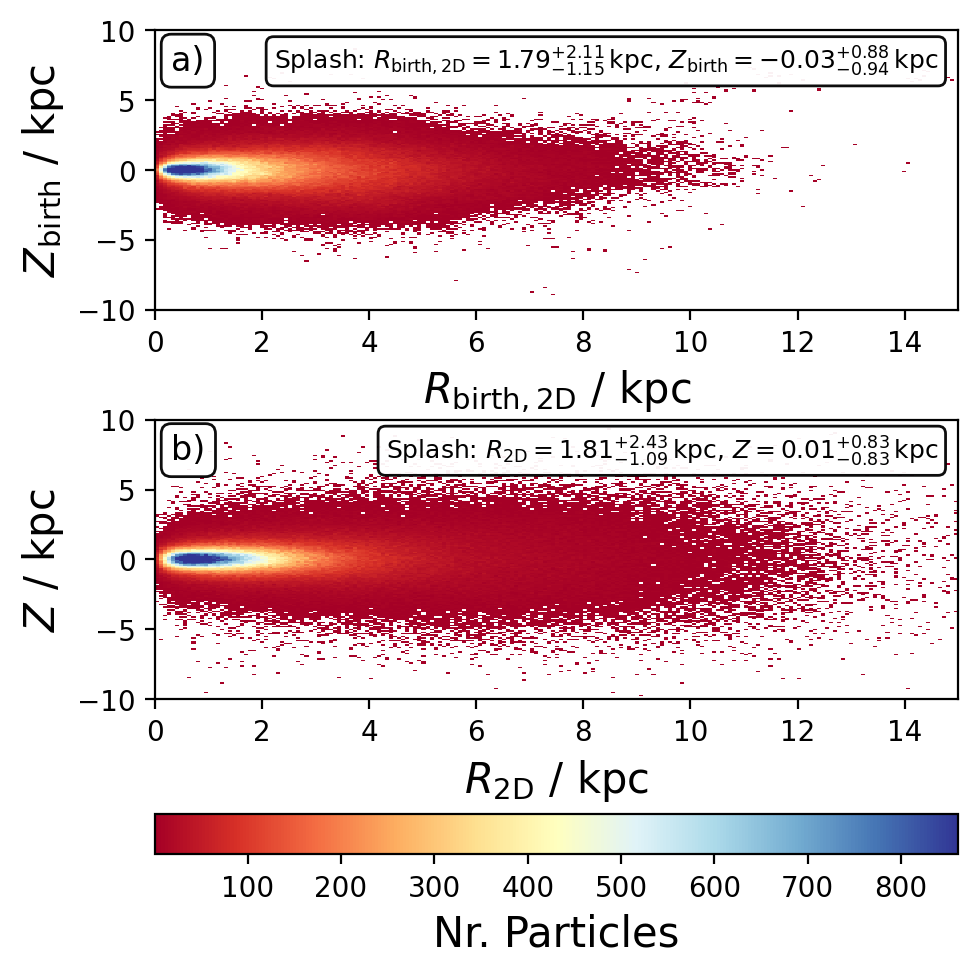
\includegraphics[width=\columnwidth]{figures/splash_rz_birth_now.png}
    \caption{Radial and vertical distribution of Splash stars. Panel a) shows birth radii $R_\mathrm{birth, 2D}$ and birth heights $Z_\mathrm{birth}$, whereas panel b) shows current radii $R_\mathrm{2D}$ and heights $Z$. Text insets show the median and 16th to 84th percentiles of each distribution
    \href{https://github.com/svenbuder/golden_thread_II/tree/main/figures}{\faGithub}.}
    \label{fig:splash_rz_birth_now}
\end{figure}

\subsection{Coeval counterparts of Splash-like stars}

In particular, we are interested in a comparison of properties of the low azimuthal velocity (Splash) stars with $V_\varphi < 75\,\mathrm{km\,s^{-1}}$ and their higher azimuthal velocity counterpart. We show their distribution in a [Fe/H] vs. $V_\varphi$ diagram in Fig.~\ref{fig:splash_vphi_distribution} and notice that their distribution both in 2-dimensions as well as each individual dimension appear rather smooth. In particular the distribution in $V_\varphi$ appears normal-distributed with a slight positive skewness, $V_\varphi = 73_{-59}^{+74}\,\mathrm{km\,s^{-1}}$%. We have thus used the \textsc{skewnorm} functionality of the \textsc{scipy.stats} module \citep{Scipy} to fit a skewed normal distribution to the data, finding a distribution around $79 \pm 65\,\mathrm{km\,s^{-1}}$ with a positive skewness of $\gamma_1$ between 0.35 and 0.51 when using \textsc{skew} or \textsc{skewnorm}, respectively. In addition, we have also looked into the chemical enrichment of the low- and high-$V_\varphi$ samples, in particular [Al/Fe] and [Mg/Mn]. The samples are visually congruent with each other (see inset of Fig.~\ref{fig:splash_alfe_mgmn}) and distributed in the region of Fig.~\ref{fig:splash_alfe_mgmn} of sample D. To statistically assess whether the two 2-dimensional distributions are drawn from the same underlying population, we apply the Maximum Mean Discrepancy test \citep{Gretton2012} using the \textsc{hyppo} package's \textsc{ksample.MMD} \citep{hyppo}. The resulting test statistic of $10^{-6}$ with a $p$-value of 0.26 indicates no significant difference between the two samples. For reference, Kolmogorov–Smirnov tests \citep{Hodges1958} applied independently to the 1D marginals via \textsc{scipy.stats.ks\_2samp} also yield high $p$-values of 1.0 and 0.86. This leads to the conclusion that both the high $V_\varphi$ and low $V_\varphi$ Splash stars are drawn (born?) from the same distribution with a large spread in $V_\varphi$.

\begin{figure*}
    \centering
    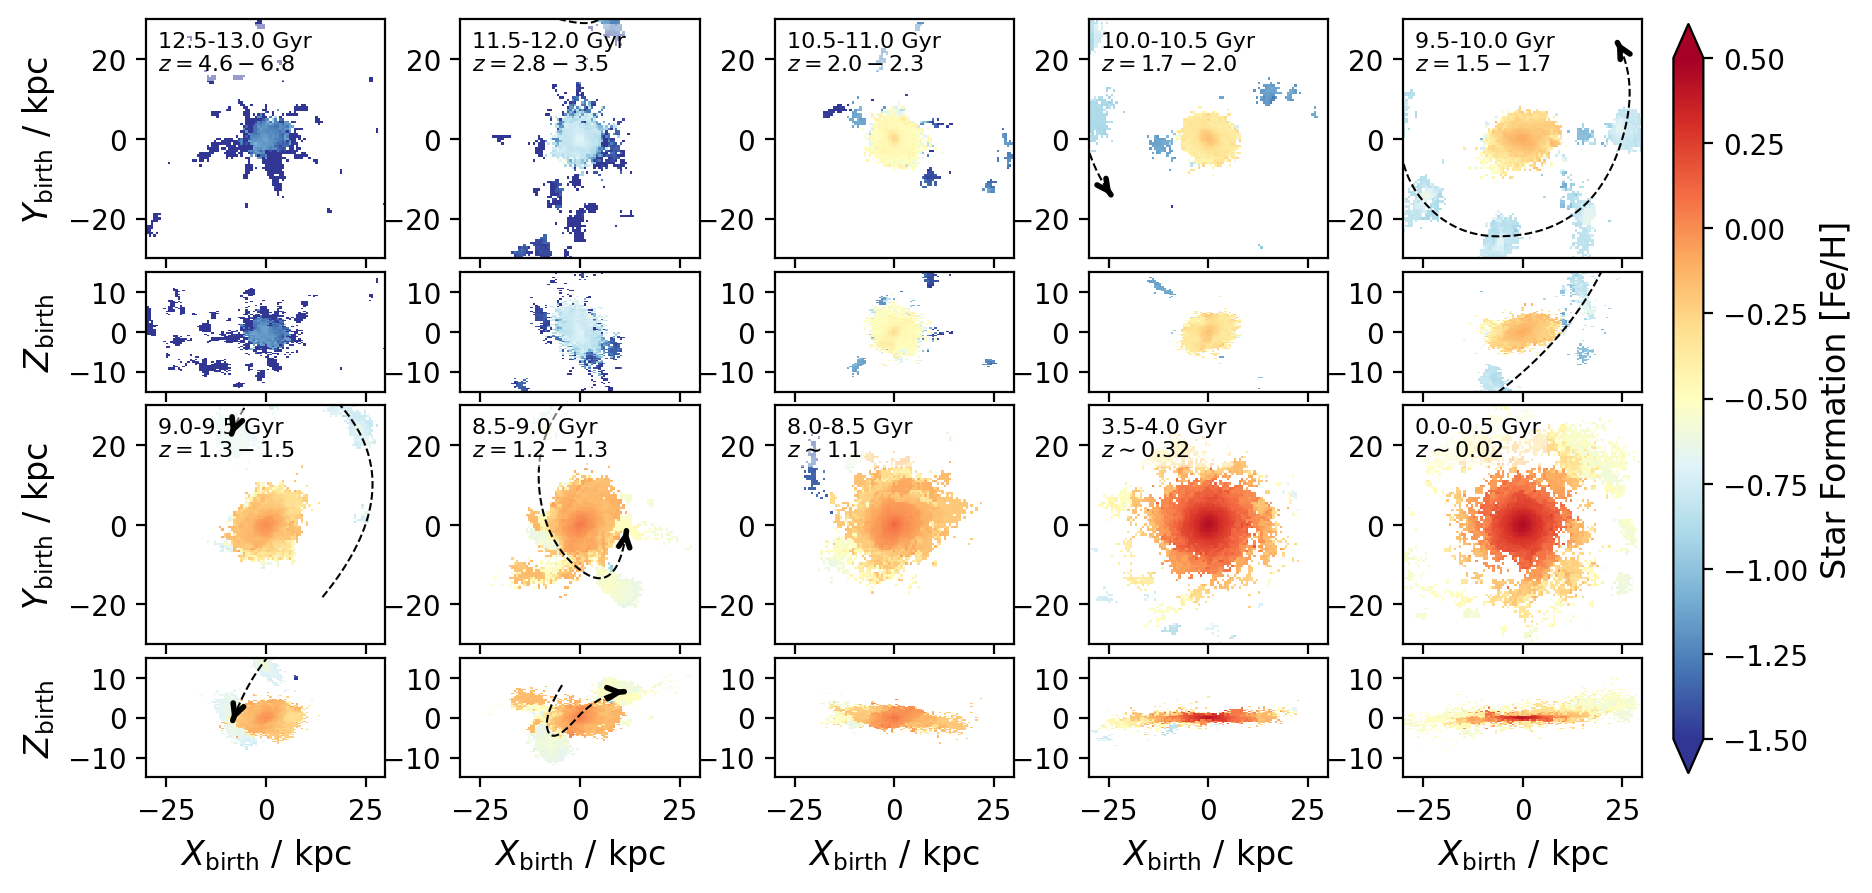
\includegraphics[width=\textwidth]{figures/trace_star_formation_xy_xz_feh_selection.png}
    \caption{Distributions of iron abundances {[Fe/H]} for the face-on ($X_\mathrm{birth}$ vs. $Y_\mathrm{birth}$, odd rows) and edge-on ($X_\mathrm{birth}$ vs. $Z_\mathrm{birth}$, even rows) views in ten selected birth epochs within $0.5\,\mathrm{Gyr}$, starting from $12.5-13.0\,\mathrm{Gyr}$ in the top-left panel to $0.0-0.5\,\mathrm{Gyr}$ in the bottom-right panel. Dashed black arrows indicate the path of the last major merger. See \href{https://github.com/svenbuder/golden_thread_II/tree/main/figures}{\faGithub} for figures with all epochs as well as colouring by density.}
    \label{fig:trace_star_formation_xy_xz_feh_selection}
\end{figure*}

\subsection{Birth and present-day orbits of Splash-like stars}

To further establish, where -- and by proxy on which orbits -- the Splash stars were born, we analyse their and the other samples' birth positions in Fig.~\ref{fig:splash_rbirth_zbirth}. The simulation makes remarkable predictions about the origin of stars that are currently residing in a small Solar neighbourhood-like region, with stars visiting from the centre of the galaxy or its furthest outskirts at $20\,\mathrm{kpc}$ (see Fig.~\ref{fig:splash_rbirth_zbirth}a) -- not to mention the accreted stars born even further away (Fig.~\ref{fig:splash_rbirth_zbirth}f). In agreement with radial migration models \citep[for example][]{Frankel2018, Frankel2020}, a significant amount of metal-rich stars (Fig.~\ref{fig:splash_rbirth_zbirth}b) is visiting from the inner galaxy (Sample B with 5-95th percentiles of $R_\mathrm{birth, 2D} \sim 3.9 - 8.9\,\mathrm{kpc}$ centred around a median of $6.3\,\mathrm{kpc}$), while high-$V_\varphi$ stars with Solar-like iron abundances (Sample C) show a larger distribution of birth origins along the disc ($R_\mathrm{birth, 2D} \sim 3.5-12.5\,\mathrm{kpc}$, centred around $7.4\,\mathrm{kpc}$). However, both the in-situ Splash ($R_\mathrm{birth, 2D} \sim 2.2-7.8\,\mathrm{kpc}$, centred around $4.6\,\mathrm{kpc}$) and the in-situ metal-poor stars ($R_\mathrm{birth, 2D} \sim 1.0-9.7\,\mathrm{kpc}$, centred around $2.9\,\mathrm{kpc}$) are basically born exclusively in the inner galaxy ($R_\mathrm{birth, 2D} \ll 8.2\,\mathrm{kpc}$) and with a larger spread of $Z_\mathrm{birth}$, that is, not on a thinner disc.

Since the Splash stars were born further inwards, the question arises, whether they were born on more radially eccentric orbits which reach into our Solar neighbourhood, or if their orbits have significantly changed through the radial splashing that shifts their initially inner orbits to overlap with our Solar neighbourhood. Because our snapshot at redshift $z = 0$ only includes the present-day velocities, we turn to a comparison of birth and present-day spatial distribution in Fig.~\ref{fig:splash_rz_birth_now} in an effort to quantify the change of spatial distributions which would imply a change of orbits. When comparing the birth (upper panel) with present-day (lower panel) density distributions in linear density, we note a more extended low-density envelope to higher radii. Similarly, we note an extend of larger $Z$-coverage for $R_\mathrm{2D} > 6\,\mathrm{kpc}$ -- again with very low densities. The overall distribution of stars has, however, changed insignificantly. This is evident in the only minor change of the average $R_\mathrm{birth,2D} = 1.79_{-1.15}^{+2.11}\,\mathrm{kpc}$% to $R_\mathrm{2D} = 1.81_{-1.09}^{+2.43}\,\mathrm{kpc}$% and $Z_\mathrm{birth} = -0.03_{-0.94}^{+0.88}\,\mathrm{kpc}$% to $Z = 0.01_{-0.83}^{+0.83}\,\mathrm{kpc}$%. When calculating the average of the change for the individual stars, we find $\overline{\Delta R_\mathrm{2D}} = \overline{R_\mathrm{2D,birth} - R_\mathrm{2D}} = -0.1_{-1.2}^{+1.1}\,\mathrm{kpc}$% and $\overline{\Delta |Z|} = \overline{|Z_\mathrm{birth}| - |Z|} = 0.03_{-0.68}^{+0.70}\,\mathrm{kpc}$%. In our particular Milky Way analogue simulation, this thus implies little orbit change of these stars, or no significant splashing, with a possible exception of stars beyond $R_\mathrm{2D} > 3.9\,\mathrm{kpc}$, the outermost $16\,\mathrm{\%}$ of Splash stars (the 84th percentile of $R_\mathrm{birth,2D}$). We discuss the implications of this finding in Section~\ref{sec:discussion}.

\subsection{Effect on newly forming stars}

Although the main focus of our study is to understand the properties and origin of the Splash, we want to briefly investigate the potential of the available birth positions to study the evolution of the main galaxy's density and chemical enrichment during and after the merging. For this purpose, we investigate the change of iron abundance [Fe/H] in birth positions in both the $X_\mathrm{birth}$ vs. $Y_\mathrm{birth}$ and $X_\mathrm{birth}$ vs. $Z_\mathrm{birth}$ dimensions in Fig.~\ref{fig:trace_star_formation_xy_xz_feh_selection}, with each panel showing the median iron abundance in each bin for stars formed within a selection of 10 star formation epochs that each span $0.5\,\mathrm{Gyr}$. We remind ourselves that because birth positions are estimated in $0.1\,\mathrm{Gyr}$ steps, we expect the footprint of the major accretion to mimic up to five smaller galaxies, which in fact are showing the position of the same smaller galaxy in $0.1\,\mathrm{Gyr}$ steps (see especially the panels around $9.5-10.0\,\mathrm{Gyr}$ in these figures).

From these figures we can assess that the stars of the early main galaxy were born on typically random orbits leading to a spheroidal galaxy shape and new stars following similar orbits until a lookback time of $\sim 10\,\mathrm{Gyr}$. Between $\sim10$ and $\sim 8.5\,\mathrm{Gyr}$ ago, we then see the birth positions follow a more and more disc-like structure with increasing radii and decreasing heights. For ages below $8\,\mathrm{Gyr}$, we then see star formation occurring within a rotationally supported disc. These observations are in agreement with the modelling by \citet{MCM2013}. Albeit qualitatively in agreement with the description of the \textit{spin-up} by \citet{Belokurov2022}, we would place the tracers of the spin-up phase exactly at the position of the Splash in the $\mathrm{[Fe/H]}$ vs. $V_\varphi$, not only more metal-poor than the Splash as done by \citet[][see their Fig.~5b]{Belokurov2022}. A detailed assessment of how the smaller galaxy’s gravitational influence and angular momentum transfer between $\sim10$ and $\sim8.6\,\mathrm{Gyr}$ contributed to the spin-up of the Milky Way analogue’s disc requires tracing gas and dark matter in addition to stars, which we leave to future work.

What we can investigate, however, is the change of star formation [Fe/H] during this time. This property is used as colour-coding for the different star formation epochs in Fig.~\ref{fig:trace_star_formation_xy_xz_feh_selection}. Here we see that after the initial main galaxy started forming stars with $\mathrm{[Fe/H]} \leq -1.5$ (dark blue), its core quickly started forming more metal-rich stars with the star formation $\mathrm{[Fe/H]}$ in the core rising from $-1.0$ to $-0.75$ between $\sim 12.5$ and $\sim11.5\,\mathrm{Gyr}$ ago, while several smaller amounts of metal-poor stars ($\mathrm{[Fe/H]} \leq -1.5$) where born outside of the core galaxy and quickly accreted. This process continues with star formation in the core reaching $\mathrm{[Fe/H]} \sim -0.2$ and the outskirts reaching $-0.35$ at a lookback time of $\sim 10\,\mathrm{Gyr}$. At this time, we notice the arrival of the major merger galaxy to within $30\,\mathrm{kpc}$ distance. Its path is indicated with dashed arrows as it continues to form stars in each $0.1\,\mathrm{Gyr}$ snapshot and finally merge with the main galaxy in a spiral pattern around $8.6\,\mathrm{Gyr}$ ago. For this galaxy, we also note a negative metallicity gradient from core to outskirts, but at lower metallicities than the main galaxy, in particular in the top-right panel of Fig.~\ref{fig:trace_star_formation_xy_xz_feh_selection}. Such gradients were also found by other simulation studies \citep{Amarante2022, Khoperskov2023d, Mori2024, Carrillo2025}. Most importantly, we notice that while the metallicity of the major merger galaxy tends to still increase and reach $\mathrm{[Fe/H]} \sim -0.5$ until $\sim 8.5\,\mathrm{Gyr}$ ago, the main galaxy's star formation [Fe/H] seems to not decrease within the inner $R_\mathrm{birth,2D} < 10\,\mathrm{kpc}$ (compare the snapshots of $8.5-9.0\,\mathrm{Gyr}$ with $8.0-8.5\,\mathrm{Gyr}$ for that region). Only in the outskirts of the galaxy at $10 \lesssim R_\mathrm{birth, 2D} \lesssim 20\,\mathrm{kpc}$ do we note some patches of lower star formation [Fe/H]. We note that \citet{Buck2023} found considerable dips in the gas metallicity [Fe/H] of this simulation during the merger. By comparison with the positions of the major merger galaxy around this time (see Fig.~9b from \citetalias{Buder2025c}), we can confirm those as accreted structures as well. This again underlines our impression of no significant lowering of star formation [Fe/H] during the merger. For all remaining epochs, we only notice a rather uneventful inside-out star formation with a radial metallicity gradient \citep[see also][]{Buder2025}.

%%%%%%%%%%%%%%%%%%%%%%%%%%%%%%%%%%%%%%%%%%%%%%%%%
%%%%%%%%%%%%%%%%%%%%%%%%%%%%%%%%%%%%%%%%%%%%%%%%%
\section{Discussion}
\label{sec:discussion}

In \citetalias{Buder2025c}, we examined the efficiency of recovering accreted stars in integral-of-motion space and assessed how much information about their birth positions and chemistry is preserved. Here, we extend this framework to focus on what can be inferred from birth positions, ages, and chemistry about the dynamical state of the early disc, and in particular on the proposed splashing of the Milky Way's protodisc \citep{Belokurov2020}.

\subsection{The nature of Splash-like stars}

Our analysis of Splash-like stars in a Solar-like neighbourhood with low azimuthal velocities and subsolar metallicities (Figs.~\ref{fig:splash_feh_vphi}--\ref{fig:splash_rz_birth_now}) suggests that these stars represent the ancient portion of the protodisc, in line with earlier observational studies \citep{Bonaca2017, Haywood2018b, DiMatteo2019, Gallart2019, Belokurov2020}. Similar to \citet{Belokurov2020}, we find that the properties of these stars bridge smoothly to those of the thick disc. However, when comparing stars with similar chemistry and ages, we also identify prograde counterparts with high $V_\varphi$, and that the $V_\varphi$ distribution of the sample shows a positive skewness (Fig.~\ref{fig:splash_vphi_distribution}). This indicates that the majority of stars in this population already occupy lower $V_\varphi$ orbits, rather than being drawn from a dynamically cold distribution that was later heated. The latter would lead to a negative skewness with a higher mean $V_\varphi$, which is inconsistent with our findings.

This challenges the interpretation that the Splash is simply the tail of a cold protodisc violently heated by \textit{GSE} \citep{DiMatteo2019, Belokurov2020}. Instead, our findings align more closely with the results of \citet{Amarante2020}, who showed in an isolated clumpy disc simulation that stars can be \emph{born hot} on halo-like orbits while retaining thick-disc chemistry. Our analysis of birth positions strengthens this view: we find no significant radial or vertical displacement between average present-day and birth positions ($\overline{\Delta R_\mathrm{2D}} = \overline{R_\mathrm{2D,birth} - R_\mathrm{2D}} = -0.1_{-1.2}^{+1.1}\,\mathrm{kpc}$%, $\overline{\Delta |Z|} = \overline{|Z_\mathrm{birth}| - |Z|} = 0.03_{-0.68}^{+0.70}\,\mathrm{kpc}$%), questioning the need for a large-scale dynamical splashing event.

\subsection{Implications for disc heating and angular momentum build-up}

The galaxy in which Splash stars formed was not yet rotation-dominated. In the simulation, a rotation-supported disc emerges only $\sim 9.5\,\mathrm{Gyr}$ ago, consistent with observational inferences of a gradual increase in disc rotation from 11 to 8 Gyr ago \citep[e.g.][]{MCM2013}. Whether this angular momentum build-up was causally linked to the last major merger remains uncertain. While some studies argue that \textit{GSE} heating produced the Splash \citep{Bonaca2020, DiMatteo2019}, our results suggest that at least part of the population was already dynamically hot. The reality may well involve a combination of both effects, as also hinted by cosmological simulations that show Splash-like stars arising in multiple pathways, including major mergers, retrograde minor mergers, and secular processes \citep{Quinn1993, Purcell2010, Villalobos2008, Villalobos2009, Dillamore2023, Dillamore2025, Kisku2025}. While secular processes such as bar resonances have also been shown as a possible pathway to generate Splash-like signatures \citep{Dillamore2022,Dillamore2023}, we note that the NIHAO-UHD simulation analysed here does not form a significant present-day bar \citep{Buder2025}. This makes it unlikely that bar-driven resonances are responsible for the Splash-like stars we identify at $z=0$, at least in this particular simulation.

Quantifying the merger contribution to angular momentum evolution is a broader challenge. The outcome depends on mass ratios, orbital configurations, and the timing of gas inflows \citep[e.g.][]{Lagos2017, Lagos2018}. A single simulation cannot establish causality, but suites of cosmological simulations offer promising routes forward \citep{Pillepich2019, SotilloRamos2022}. Our findings underscore the need for such systematic studies to disentangle the relative importance of heating versus hot-born origins.

\subsection{Limitations and outlook}

In this work our analysis focused solely on the stellar component, in line with current observations. We do not explicitly follow gas inflows onto the Milky Way analogue or the gas content of the Milky Way analogue and its major merger, which are known to influence the degree of mixing and subsequent star formation \citep[e.g.][]{Cooper2015, Agertz2021, Renaud2021b, Buck2023, TepperGarcia2024}. Future work combining stellar and gaseous tracers may better constrain the role of gas-rich accretion in producing stars with Splash-like properties.

As more precise observational constraints become available, particularly in ages and multi-element abundance patterns, it should become possible to further test whether Splash-like stars were primarily heated, born hot, or both. The emerging diversity of predictions across simulation suites \citep{Brooks2025} highlights the value of confronting these with observationally defined populations. Our results demonstrate that cosmological simulations with traced birth positions provide a crucial tool for this task, moving beyond kinematics alone and towards a more nuanced understanding of the Splash as a window into the Milky Way’s early disc and merger history.

%%%%%%%%%%%%%%%%%%%%%%%%%%%%%%%%%%%%%%%%%%%%%%%%%
%%%%%%%%%%%%%%%%%%%%%%%%%%%%%%%%%%%%%%%%%%%%%%%%%
\section{Conclusions}
\label{sec:conclusions}

In \citetalias{Buder2025c}, we established the framework for interpreting the last major merger of a Milky Way analogue, focusing on selection efficiency and the retention of chemodynamical memory. Here, we have used the same NIHAO-UHD simulation to examine the proposed Splash population, enabled by tracing the birth positions, ages, and chemistry of stars.

Our analysis finds no significant evidence for a large-scale dynamical splashing of in-situ stars. Instead, protodisc stars -- including those with present-day low azimuthal velocities -- were already born on dynamically hot orbits in a turbulent early disc. The transition to a rotation-supported disc occurs only during or after the merger. This suggests that much of the observed Splash may not require violent heating by the \textit{GSE} merger, but can arise naturally from stars formed in a thick, kinematically hot disc, later intermixed with accreted stars and stars formed from merger-driven gas inflows.

These results place our simulation in closer agreement with models in which Splash-like populations are \emph{born hot} in a turbulent disc\citep[e.g.][]{Amarante2020}, during the spin-up phase \citep[e.g.][]{Yu2023}, possibly shaped by feedback-driven \textit{baryon sloshing} in gas-rich progenitors \citep{BlandHawthorn2025}, while still acknowledging that merger-induced heating may contribute, as argued by other studies \citep[e.g.][]{DiMatteo2019, Belokurov2020, Bonaca2020}. Together with recent evidence from cosmological simulations and observations \citep{Dillamore2022, Dillamore2023, Khoperskov2023, Dillamore2025, Kisku2025}, this highlights that Splash-like stars likely arise through a combination of pathways rather than a single mechanism.

We conclude that the interpretation of the Splash as a distinct, merger-heated population is overly restrictive. A more nuanced view is required, in which kinematics, chemistry, and formation history jointly contribute to the observed distribution of stars. Cosmological simulations with birth-position information provide a critical benchmark for disentangling these processes, and future simulation suites will be essential for quantifying the balance between heated and born-hot origins in the context of the Milky Way’s early assembly.

% \clearpage
%%%%%%%%%%%%%%%%%%%%%%%%%%%%%%%%%%%%%%%%%%%%%%%%%
%%%%%%%%%%%%%%%%%%%%%%%%%%%%%%%%%%%%%%%%%%%%%%%%%
\section*{Acknowledgments}

We acknowledge the traditional owners of the land on which the ANU stands, the Ngunnawal and Ngambri people. We pay our respects to elders past, and present and are proud to continue their tradition of surveying the night sky and its mysteries to better understand our Universe. SB acknowledges support from the Australian Research Council under grant number DE240100150.
TB's contribution to this project was made possible by funding from the Carl Zeiss Stiftung. \'{A}S~acknowledges funding from the European Research Council (ERC) under the European Union’s Horizon 2020 research and innovation programme (grant agreement No. 101117455).

%%%%%%%%%%%%%%%%%%%%%%%%%%%%%%%%%%%%%%%%%%%%%%%%%
%%%%%%%%%%%%%%%%%%%%%%%%%%%%%%%%%%%%%%%%%%%%%%%%%
\section*{Data Availability}

All code to reproduce the analysis and figures can be publicly accessed via \url{https://github.com/svenbuder/golden_thread_II}.
The used simulation snapshot can be publicly accessed as FITS file via \url{https://github.com/svenbuder/preparing_NIHAO}. Original data, more snapshots and other galaxies can be found at \url{https://tobias-buck.de/#sim_data}. We encourage interested readers to get in contact with the authors for full data access and advice for use and cite \citet{Buck2020b, Buck2021}.

\section*{Software}

The research for this publication was coded in \textsc{python} (version 3.12.11) and included its packages
\textsc{astropy} \citep[v. 7.1.0;][]{Robitaille2013,PriceWhelan2018},
\textsc{hyppo} \citep[v. 0.5.2;][]{hyppo},
\textsc{IPython} \citep[v. 9.1.0;][]{ipython},
\textsc{matplotlib} \citep[v. 3.10.3;][]{matplotlib},
\textsc{NumPy} \citep[v. 2.2.6;][]{numpy}, as well as
\textsc{scipy} \citep[v. 1.16.0;][]{Scipy}.
We used \textsc{topcat} \citep[v. 4.7;][]{Taylor2005}.

%%%%%%%%%%%%%%%%%%%%%%%%%%%%%%%%%%%%%%%%%%%%%%%%%
%%%%%%%%%%%%%%%%%%%%%%%%%%%%%%%%%%%%%%%%%%%%%%%%%
\bibliographystyle{mnras}
\bibliography{bib}

%%%%%%%%%%%%%%%%%%%%%%%%%%%%%%%%%%%%%%%%%%%%%%%%%
%%%%%%%%%%%%%%%%%%%%%%%%%%%%%%%%%%%%%%%%%%%%%%%%%
% \clearpage
%\appendix

% \bsp
\label{lastpage}
\end{document}